\documentclass[a4paper,twocolumn]{article}
\usepackage{fontspec}   %加這個就可以設定字體
\usepackage{xeCJK}       %讓中英文字體分開設置
\usepackage{indentfirst}
\usepackage{listings}
\usepackage[newfloat]{minted}
\usepackage{float}
\usepackage{graphicx}
\usepackage{caption}
\usepackage{fancyhdr}
\usepackage{hyperref}
\usepackage{amsmath}
\usepackage{multirow}
\usepackage[dvipsnames]{xcolor}
\usepackage{graphicx}
\usepackage{tabularx}
\usepackage{booktabs}
\usepackage{caption}
\usepackage{subcaption}
\usepackage{pifont}
\usepackage{amssymb}
\usepackage[backend=biber]{biblatex}
\addbibresource{main.bib}


\usepackage{pdftexcmds}
\usepackage{catchfile}
\usepackage{ifluatex}
\usepackage{ifplatform}

\usepackage[breakable, listings, skins, minted]{tcolorbox}
\usepackage{etoolbox}
\setminted{fontsize=\footnotesize}
\renewtcblisting{minted}{%
    listing engine=minted,
    minted language=python,
    listing only,
    breakable,
    enhanced,
    minted options = {
        linenos, 
        breaklines=true, 
        breakbefore=., 
        % fontsize=\footnotesize, 
        numbersep=2mm
    },
    overlay={%
        \begin{tcbclipinterior}
            \fill[gray!25] (frame.south west) rectangle ([xshift=4mm]frame.north west);
        \end{tcbclipinterior}
    }   
}

\usepackage[
top=1.5cm,
bottom=0.75cm,
left=1.5cm,
right=1.5cm,
includehead,includefoot,
heightrounded, % to avoid spurious underfull messages
]{geometry} 

\newenvironment{code}{\captionsetup{type=listing}}{}
\SetupFloatingEnvironment{listing}{name=Code}



\title{Deep Learning Lab 7 -- Policy-based Reinforcement Learning}
\author{110550088 李杰穎}
\date{\today}


\setCJKmainfont{Noto Serif TC}



\ifwindows
\setmonofont[Mapping=tex-text]{Consolas}
\fi

\XeTeXlinebreaklocale "zh"             %這兩行一定要加,中文才能自動換行
\XeTeXlinebreakskip = 0pt plus 1pt     %這兩行一定要加,中文才能自動換行

\newcommand*{\dif}{\mathop{}\!\mathrm{d}}

\begin{document}
\maketitle
\section{Introduction}

In this lab, I implement two policy-based reinforcement learning algorithms: Advantage Actor-Critic (A2C)\cite{mnih2016asynchronous} and Proximal Policy Optimization (PPO)\cite{schulman2017proximal} with Generalized Advantage Estimation (GAE). These algorithms are applied to solve two distinct control tasks with continuous action spaces: Pendulum-v1 and Walker2d-v4.

The Pendulum-v1 is a classic control problem where the objective is to swing up and stabilize an inverted pendulum in an upright position. This environment has a simple 3-dimensional state space representing the pendulum's position and angular velocity, and a 1-dimensional continuous action space for applying torque to the pendulum within the range of [-2, 2].

The Walker2d-v4 presents a more complex challenge involving a planar biped robot that must learn to walk forward without falling. This environment features a higher-dimensional state space and a 6-dimensional continuous action space controlling various joint torques, making it significantly more difficult to solve than the Pendulum environment.

My implementation explores how policy-based methods, which directly optimize the policy function through stochastic policy gradients, can effectively solve these continuous control tasks. The Gaussian policy is employed to sample continuous actions while promoting adequate exploration. I compare the performance of A2C and PPO, analyzing their sample efficiency and training stability, and examine the impact of key hyperparameters such as the clipping parameter and entropy coefficient on learning performance.

Through these experiments, I demonstrate how modern policy optimization methods like PPO can effectively solve complex locomotion tasks, highlighting the benefits of PPO's improved stability and sample efficiency over more traditional approaches like A2C.

\section{Implementation Details}

\subsection{Advantage Actor-Critic (A2C)}

A2C combines policy gradient with value-based methods using two neural networks: an actor that determines actions through a stochastic policy, and a critic that evaluates states with a value network.

\paragraph{Policy Network.} I implemented the actor network as a Gaussian policy that outputs the mean action and uses a learnable standard deviation parameter for stochastic action sampling:

\begin{code}
\captionof{listing}{\textbf{Actor Network Implementation}}
\begin{minted}
class Actor(nn.Module):
    def __init__(self, in_dim: int, out_dim: int, hidden_dim: int = 128, activation=nn.Tanh):
        """Initialize."""
        super(Actor, self).__init__()
        
        self.fc1 = nn.Linear(in_dim, hidden_dim)
        self.fc2 = nn.Linear(hidden_dim, hidden_dim)
        self.mean_layer = nn.Linear(hidden_dim, out_dim)
        self.activation = activation()
        # Learnable log standard deviations
        self.logstds = nn.Parameter(torch.full((out_dim,), 0.5))

    def forward(self, state: torch.Tensor) -> Tuple[torch.Tensor, Normal]:
        """Forward method implementation."""
        x = self.activation(self.fc1(state))
        x = self.activation(self.fc2(x))
        means = self.mean_layer(x)
        
        # Constrain standard deviations to reasonable range
        stds = torch.clamp(torch.exp(self.logstds), 1e-5, 3.0)
        
        # Create normal distribution
        dist = Normal(means, stds)
        action = dist.sample()

        return action, dist
\end{minted}
\end{code}

The network uses Tanh as the activation function. For action selection, I apply a tanh transformation and scaling to constrain actions to the proper range for the Pendulum environment ([-2, 2]).

\paragraph{Critic Network.} The critic network estimates the state-value function, which is used to compute the advantage function:

\begin{code}
\captionof{listing}{\textbf{Critic Network Implementation}}
\begin{minted}
class Critic(nn.Module):
    def __init__(self, in_dim: int, hidden_dim: int = 128, activation=nn.Tanh):
        """Initialize."""
        super(Critic, self).__init__()

        self.fc1 = nn.Linear(in_dim, hidden_dim)
        self.fc2 = nn.Linear(hidden_dim, hidden_dim)
        self.fc3 = nn.Linear(hidden_dim, 1)
        self.activation = activation()
        
    def forward(self, state: torch.Tensor) -> torch.Tensor:
        """Forward method implementation."""
        x = self.activation(self.fc1(state))
        x = self.activation(self.fc2(x))
        value = self.fc3(x)
        return value
\end{minted}
\end{code}

\paragraph{Advantage Estimation.} For A2C, I implemented both one-step TD-error advantage estimation and the option to use full Monte Carlo returns for more stable training:

\begin{code}
\captionof{listing}{\textbf{Advantage Estimation in A2C}}
\begin{minted}
# TD-error for advantage estimation
if self.use_mc_returns:
    # Monte Carlo returns (use if trajectory is complete)
    with torch.no_grad():
        R = self.critic(next_states[-1]) * (1 - dones[-1])  # Zero if terminal

    returns = []
    for r, d in zip(reversed(rewards), reversed(dones)):
        R = r + self.gamma * R * (1 - d)
        returns.insert(0, R)
    td_targets = torch.cat(returns, dim=0)
else:
    # TD targets (bootstrapping)
    with torch.no_grad():
        td_targets = rewards + self.gamma * self.critic(next_states) * (1 - dones)

values = self.critic(states)
advantage = (td_targets - values).detach()
\end{minted}
\end{code}

\paragraph{Policy Gradient with Advantage.} The A2C policy gradient is computed using the log probability of the action multiplied by the advantage:

\begin{code}
\captionof{listing}{\textbf{A2C Policy Update}}
\begin{minted}
# Get action distributions
_, dists = self.actor(states)
log_probs = dists.log_prob(actions)
entropies = dists.entropy()

# Calculate actor loss with entropy regularization for exploration
actor_loss = (-log_probs * advantage).mean() - self.entropy_weight * entropies.mean()

# Calculate critic loss
value_loss = F.smooth_l1_loss(values, td_targets)

# Update actor
self.actor_optimizer.zero_grad()
actor_loss.backward()
torch.nn.utils.clip_grad_norm_(self.actor.parameters(), 0.5)
self.actor_optimizer.step()

# Update critic
self.critic_optimizer.zero_grad()
value_loss.backward()
torch.nn.utils.clip_grad_norm_(self.critic.parameters(), 0.5)
self.critic_optimizer.step()
\end{minted}
\end{code}

I integrate two components in order to stablize the training process:
\begin{enumerate}
\item \textbf{Huber Loss}: As discussed in Lab 5, we found that Huber loss is robust to outliers. Thus, we introduce it again in this lab
\item \textbf{Graident Clipping}: Previous literatures suggest that adding gradient clipping with a maximum norm of 0.5 
\end{enumerate}



\subsection{Proximal Policy Optimization (PPO)}

PPO\cite{schulman2017proximal} extends policy gradient methods by introducing a surrogate objective that constrains policy updates to prevent large, destructive changes. My implementation adds several improvements over A2C:

\paragraph{Clipped Surrogate Objective.} This is the core innovation in PPO, where the policy update is clipped to prevent excessive changes:

\begin{code}
\captionof{listing}{\textbf{PPO Clipped Surrogate Objective}}
\begin{minted}
# Calculate probability ratio
_, dist = self.actor(state)
log_prob = dist.log_prob(action)
ratio = (log_prob - old_log_prob).exp()

# Compute surrogate objectives
surrogate1 = ratio * adv
surrogate2 = torch.clamp(ratio, 1 - self.epsilon, 1 + self.epsilon) * adv

# Take minimum to clip the objective
actor_loss = -torch.min(surrogate1, surrogate2).mean()

# Add entropy bonus for exploration
entropy = dist.entropy().mean()
actor_loss = actor_loss - self.entropy_weight * entropy
\end{minted}
\end{code}

The clipping parameter (epsilon) limits how much the policy can change in a single update. I experimented with different values (0.1, 0.2, 0.3) to study its effect on training stability.

\paragraph{Generalized Advantage Estimation (GAE).} GAE provides a better trade-off between bias and variance in advantage estimation, improving the learning signal quality:

\begin{code}
\captionof{listing}{\textbf{GAE Implementation}}
\begin{minted}
def compute_gae(
    next_value: list, rewards: list, masks: list, values: list, gamma: float, tau: float) -> List:
    """Compute generalized advantage estimation."""

    values = values + [next_value]
    gae_returns = []
    gae = 0

    for step in reversed(range(len(rewards))):
        delta = rewards[step] + gamma * values[step + 1] * masks[step] - values[step]
        gae = delta + gamma * tau * masks[step] * gae
        gae_returns.insert(0, gae + values[step])
    
    return gae_returns
\end{minted}
\end{code}

The lambda parameter (tau) controls the trade-off between bias and variance. A value of 0.95 was used for the GAE calculation, balancing between the immediate TD advantage (λ=0) and the full Monte Carlo advantage (λ=1).

\paragraph{Batch Collection and Mini-batch Updates.} PPO requires collecting a batch of experiences before updating the policy, enabling multiple gradient updates on the same data:

\begin{code}
\captionof{listing}{\textbf{PPO Sample Collection and Batch Updates}}
\begin{minted}
# Memory for training
self.states: List[torch.Tensor] = []
self.actions: List[torch.Tensor] = []
self.rewards: List[torch.Tensor] = []
self.values: List[torch.Tensor] = []
self.masks: List[torch.Tensor] = []
self.log_probs: List[torch.Tensor] = []

# In the training loop
for _ in range(self.rollout_len):
    action = self.select_action(state)
    next_state, reward, done = self.step(action)
    # State, action, reward, etc. are stored in the memory

# After collecting a batch, perform multiple updates
for state, action, old_value, old_log_prob, return_, adv in ppo_iter(
    update_epoch=self.update_epoch,
    mini_batch_size=self.batch_size,
    states=states,
    actions=actions,
    values=values,
    log_probs=log_probs,
    returns=returns,
    advantages=advantages,
):
    # Update actor and critic networks using mini-batches
\end{minted}
\end{code}

I use a large rollout length (64 for Pendulum, 2048 for Walker) to collect sufficient data before updating, and then perform multiple epochs of updates (10) on this data, with each epoch processing multiple mini-batches.

\subsection{Modifications for Walker2d-v4}

For the more complex Walker2d-v4 environment, I made several modifications to the PPO implementation:

\paragraph{Larger Network Architecture.} The network architecture was expanded to handle the increased complexity:

\begin{code}
\captionof{listing}{\textbf{Walker Architecture}}
\begin{minted}
# Actor network for Walker2d
self.fc1 = nn.Linear(in_dim, 256)
self.fc2 = nn.Linear(256, 256)
self.fc3 = nn.Linear(256, 128)
self.mu = nn.Linear(128, out_dim)

# Critic network for Walker2d
self.fc1 = nn.Linear(in_dim, 256)
self.fc2 = nn.Linear(256, 256)
self.fc3 = nn.Linear(256, 1)
\end{minted}
\end{code}

\paragraph{State and Reward Normalization.} To improve training stability in the more complex environment, I implemented state and reward normalization:

\begin{code}
\captionof{listing}{\textbf{Observation and Reward Normalization}}
\begin{minted}
class RunningMeanStd:
    def __init__(self, epsilon=1e-4, shape=()):
        self.mean = np.zeros(shape, dtype=np.float32)
        self.var = np.ones(shape, dtype=np.float32)
        self.count = epsilon
        
    def update(self, x):
        batch_mean = np.mean(x, axis=0)
        batch_var = np.var(x, axis=0)
        batch_count = x.shape[0]
        
        self.update_from_moments(batch_mean, batch_var, batch_count)
        
    def normalize(self, x):
        return (x - self.mean) / (np.sqrt(self.var) + 1e-8)

# In the agent, when selecting actions:
if self.normalize_obs:
    state = self.obs_rms.normalize(state)
    state = np.clip(state, -self.clip_obs, self.clip_obs)

# For reward normalization:
if self.normalize_reward:
    norm_reward = reward / (np.sqrt(self.reward_rms.var) + 1e-8) * self.reward_scale
\end{minted}
\end{code}

This normalization technique keeps track of the running mean and standard deviation of observations and rewards, enabling stable learning even when the environment produces values with widely varying scales.


\subsection{Enforcing Exploration}

Despite A2C and PPO being on-policy methods, I incorporated several techniques to encourage exploration:

\begin{enumerate}
    \item \textbf{Entropy Regularization:} I added an entropy bonus to the loss function, encouraging the policy to maintain sufficient stochasticity:
    
    \begin{code}
    \captionof{listing}{\textbf{Entropy Regularization}}
    \begin{minted}
    # Add entropy bonus to encourage exploration
    entropy = dist.entropy().mean()
    actor_loss = actor_loss - self.entropy_weight * entropy
    \end{minted}
    \end{code}
    
    \item \textbf{Stochastic Action Sampling:} During training, actions are sampled from the Gaussian policy distribution rather than taking the mean action:
    
    \begin{code}
    \captionof{listing}{\textbf{Stochastic Action Selection}}
    \begin{minted}
    # Sample action from distribution during training
    action, dist = self.actor(state)
    selected_action = dist.mean if self.is_test else action
    \end{minted}
    \end{code}
    
    \item \textbf{Initial Standard Deviation:} The policy's standard deviation parameters are initialized to a relatively high value (0.5) to ensure wide exploration early in training:
    
    \begin{code}
    \captionof{listing}{\textbf{Standard Deviation Initialization}}
    \begin{minted}
    # Initialize with higher value for more exploration
    self.logstds = nn.Parameter(torch.full((out_dim,), 0.5))
    \end{minted}
    \end{code}
\end{enumerate}

\subsection{Tracking with Weights \& Biases}

I used Weights \& Biases (wandb) for experiment tracking and visualization:

\begin{code}
\captionof{listing}{\textbf{Weights \& Biases Integration}}
\begin{minted}
# Initialize WandB at the start of training
wandb.init(project="DLP-Lab7-PPO-Walker", 
           name=args.wandb_run_name, 
           save_code=True, 
           config=args)

# Log metrics during training
wandb.log({
    "train/episode": episode_count,
    "train/episodic_return": score,
    "train/episode_length": episode_length,
    "train/total_steps": self.total_step,
    "actor_loss": actor_loss,
    "critic_loss": critic_loss
})

# Track evaluation metrics
wandb.log({
    "eval/episode": episode,
    "eval/avg_reward": avg_reward,
    "eval/total_steps": self.total_step
})
\end{minted}
\end{code}

This setup allowed me to track losses, rewards, episode lengths, and other key metrics throughout training, facilitating the comparison of different algorithms and hyperparameter configurations. WandB also provided useful visualizations for the training progress and performance analysis.


\subsection{Hyperparameters}

For the hyperparameters of PPO, I mainly reference values from ~\cite{rl-zoo3}.

\subsubsection{A2C on Pendulum-v1}
\begin{itemize}
	\item Actor LR: 0.0004
	\item Critic LR: 0.004
	\item Optimizer: Adam
	\item Discount factor: 0.9
	\item Entorpy weight: 0.05
	\item Mini-batch size: 32
	\item Seed: 77
\end{itemize}
\subsubsection{PPO on Pendulum-v1}
\begin{itemize}
	\item Actor LR: 0.001
	\item Critic LR: 0.005
	\item Optimizer: Adam
	\item Discount factor: 0.9
	\item Entorpy weight: 0.01
	\item PPO Clip ratio ($\epsilon$): 0.2
	\item GAE $\tau$: 0.9
	\item Rollout length: 1024
	\item Batch size: 64
	\item Update epochs: 64
	\item Seed: 77
\end{itemize}
\subsubsection{PPO on Walker2d-v4}
\begin{itemize}
	\item Actor LR: 0.00005
	\item Critic LR: 0.0002
	\item Optimizer: Adam
	\item Discount factor: 0.99
	\item Entorpy weight: 0.01
	\item PPO Clip ratio ($\epsilon$): 0.1
	\item GAE $\tau$: 0.95
	\item Rollout length: 512
	\item Batch size: 32
	\item Update epochs: 20
	\item Seed: 77
\end{itemize}

\subsection{Random Seeds}
\subsubsection{Task 1}
\texttt{[77, 78, 80, 81, 83, 84, 86, 88, 90, 91, 94, 96, 97, 99, 103, 105, 107, 114, 115, 121]}
\subsubsection{Task 2}
\texttt{[78, 81, 83, 86, 87, 88, 89, 90, 91, 92, 94, 95, 97, 99, 103, 105, 107, 109, 121, 123]}
\subsubsection{Task 3}
\texttt{[42, 43, 44, 45, 46]}

\section{Analysis and Discussion}

\subsection{Training Curves}

\begin{figure}[H]
\centering
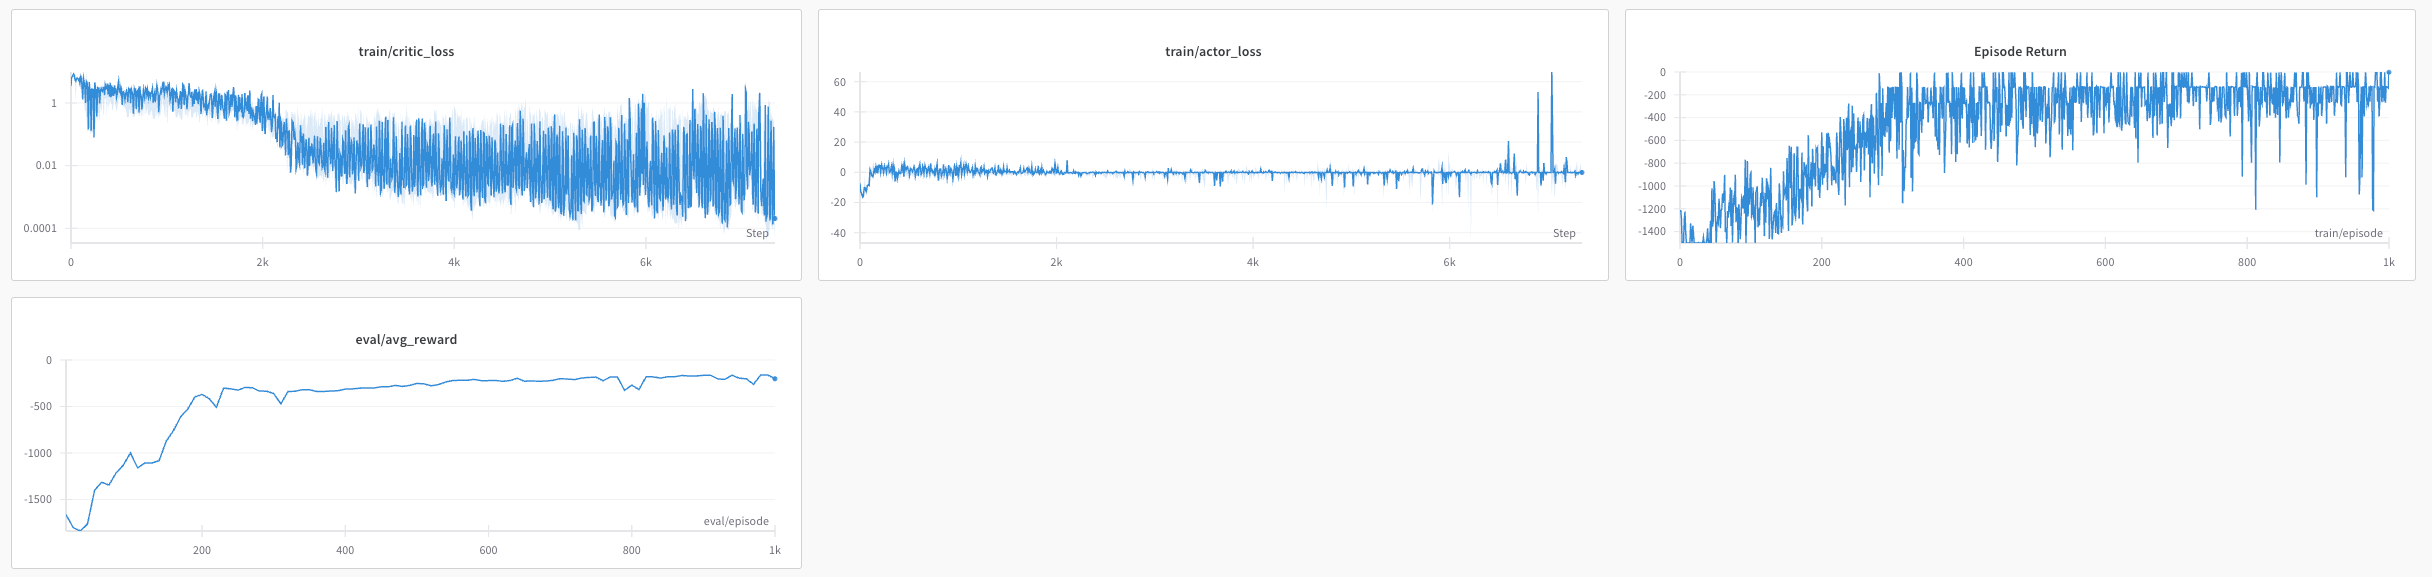
\includegraphics[width=0.95\linewidth]{figures/curve_a2c}
\caption{The traning curve of A2C on Pendulum-v1. A2C can achieve average reward around -161.}
\label{fig:curvea2c}
\end{figure}


\begin{figure}[H]
\centering
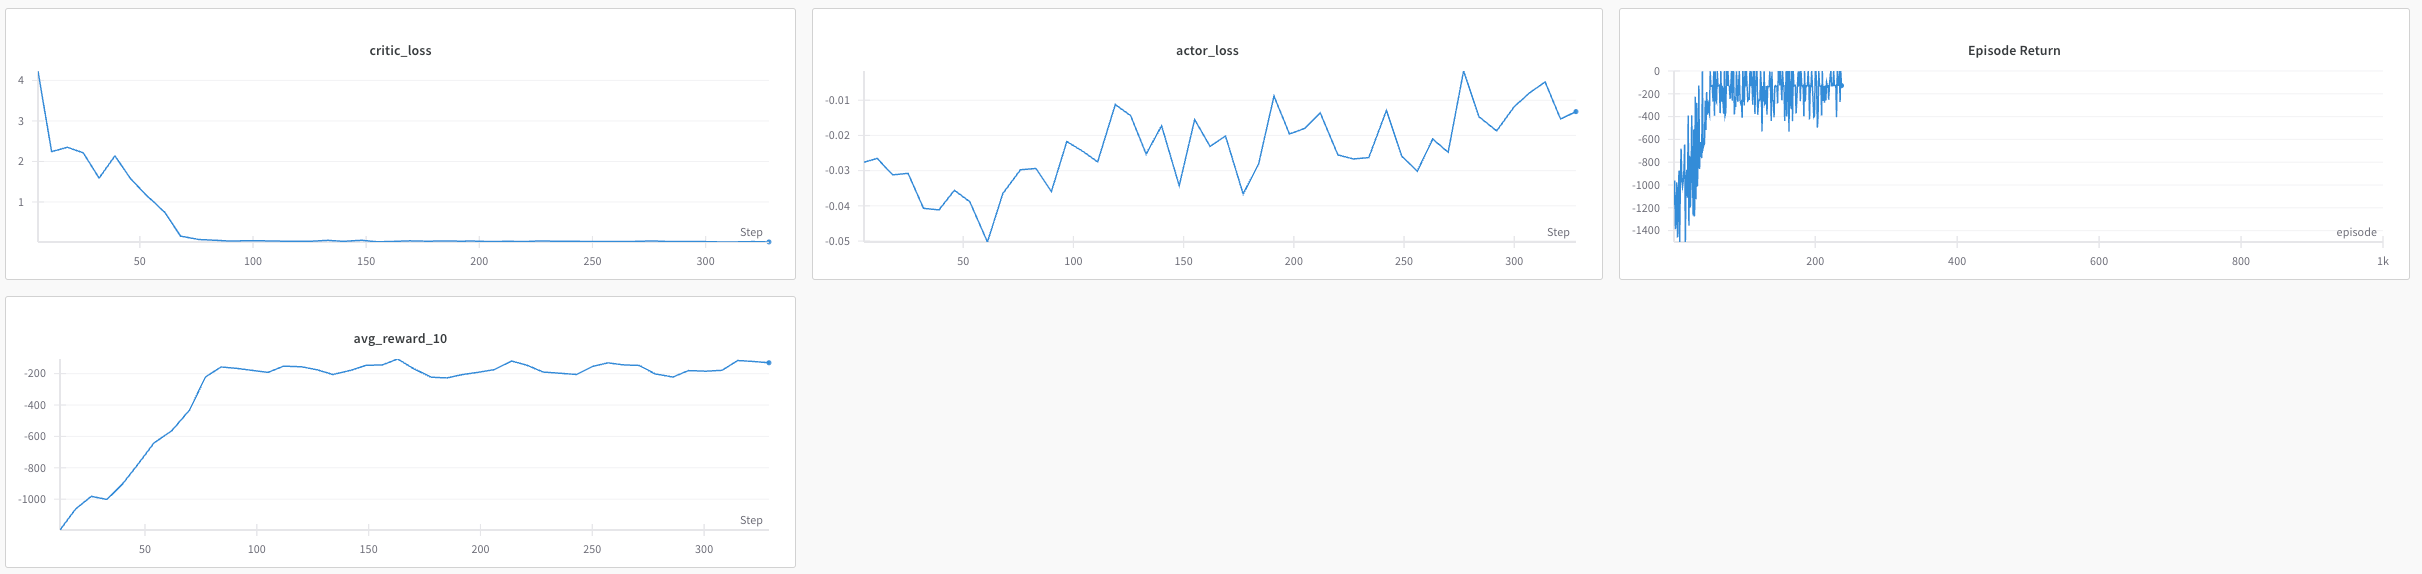
\includegraphics[width=0.95\linewidth]{figures/curve_ppo}
\caption{The training curve of PPO on Pendulum-v1. We can observe that the episode reward reaches -150 with only 30 episodes, demostrating the effectness of PPO.}
\label{fig:curveppo}
\end{figure}

\begin{figure}[H]
\centering
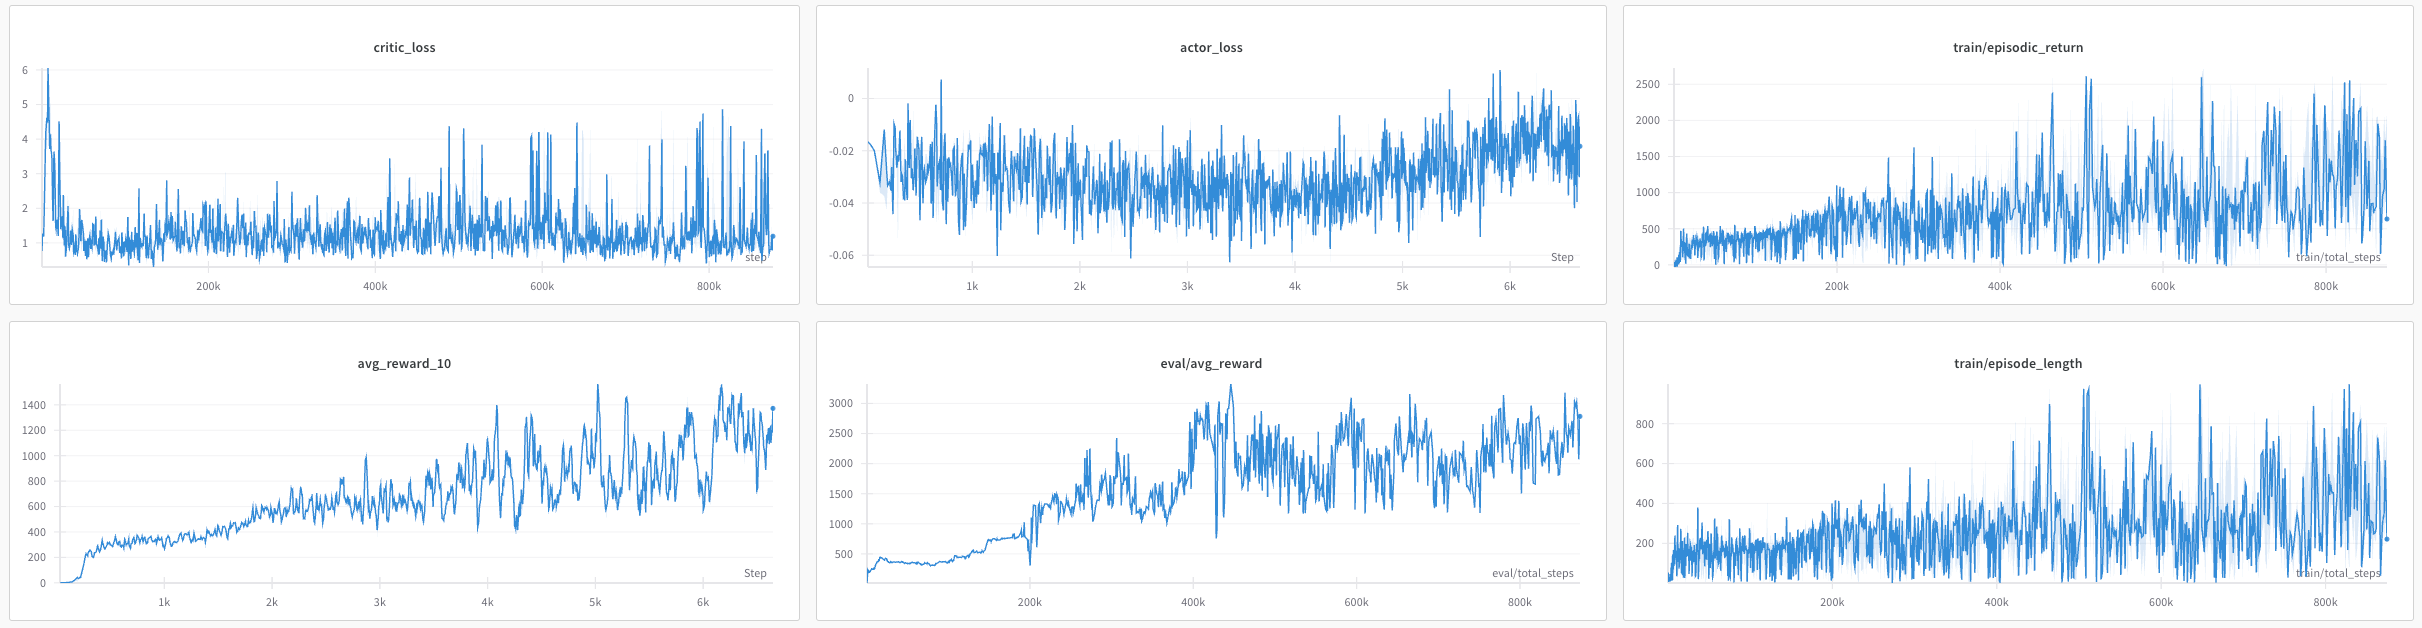
\includegraphics[width=0.95\linewidth]{figures/curve_ppo_walker}
\caption{The training curve of PPO on Walker2d-v4. We can observe that average eval episode reward reaches approximately 2500 with only 300K envrionment steps, demostrating the effectness of PPO.}
\label{fig:curveppowalker}
\end{figure}



\autoref{fig:curvea2c} and \autoref{fig:curveppo} illustrate the training progress of A2C and PPO on the Pendulum-v1 environment. The PPO algorithm demonstrates significantly faster learning and achieves higher rewards earlier in training compared to A2C. Most notably, PPO reaches a reward threshold of -150 after approximately 36 episodes, whereas A2C requires around 286 episodes to reach the same performance level. This improved sample efficiency of PPO can be attributed to its more stable policy updates through clipping and the use of multiple optimization passes on the same data.

\autoref{fig:curveppowalker} shows the training curve of PPO on Walker2d-v4. We can observe that the model can only reach around episode reward of 400 before 100K envrionment steps. However, the model suddenly learns well from the data, and starts to perform well. It reach average evaluation score around 400K environment steps. This outstanding performance showcases the ability of PPO with optimized hyperparameters.


\subsection{Sample Efficiency and Training Stability}

\begin{table}[H]
\centering
\caption{Comparison of Sample Efficiency and Training Stability for Pendulum-v1}
\label{tab:efficiency_comparison}
\begin{tabular}{lcc}
\toprule
\textbf{Algorithm} & \textbf{Episodes to -150} & \textbf{Best Reward} \\
\midrule
A2C & 286 & -161.7 \\
PPO & 36 &  -106.82 \\
\bottomrule
\end{tabular}
\end{table}

As shown in Table \ref{tab:efficiency_comparison}, PPO demonstrates superior sample efficiency, requiring approximately 87\% fewer environment steps than A2C to reach the threshold reward of -150 on the Pendulum-v1 task. This efficiency gain is a direct result of PPO's ability to perform multiple gradient updates on the same batch of data, extracting more learning signal from each collected experience.

Additionally, PPO achieves a higher final average reward (-106.82 compared to -161.7) and exhibits substantially better training stabiliy, as shown in \autoref{fig:curvea2c} and \autoref{fig:curveppo}. This improved stability is primarily due to the trust region constraint enforced by the clipping mechanism, which prevents the policy from making destructive updates that could lead to performance collapses.

For the Walker2d-v4 environment, PPO required approximately 400K steps to reach a reward of 2,500, which aligns with the task's higher complexity. The algorithm demonstrated the ability to learn effective locomotion strategies despite the challenges posed by the high-dimensional continuous control problem.

The improved performance of PPO can be attributed to several factors:

\begin{enumerate}
    \item \textbf{Trust Region Constraint:} By clipping the policy update ratio, PPO prevents excessively large policy changes that could destabilize learning, providing smoother and more consistent improvement.
    
    \item \textbf{Generalized Advantage Estimation:} GAE provides a better bias-variance trade-off in advantage estimation, leading to more stable and effective policy updates, particularly in environments with longer episodes like Walker2d.
    
    \item \textbf{Multiple Epochs per Batch:} PPO performs multiple optimization steps on the same batch of data, improving sample efficiency by extracting more learning from each collected experience.
    
    \item \textbf{Observation and Reward Normalization:} For the Walker2d environment, normalization techniques significantly improved learning stability by handling varying scales in the state and reward spaces.
\end{enumerate}

\subsection{Empirical Study on Key Parameters}

\begin{figure}[H]
\centering
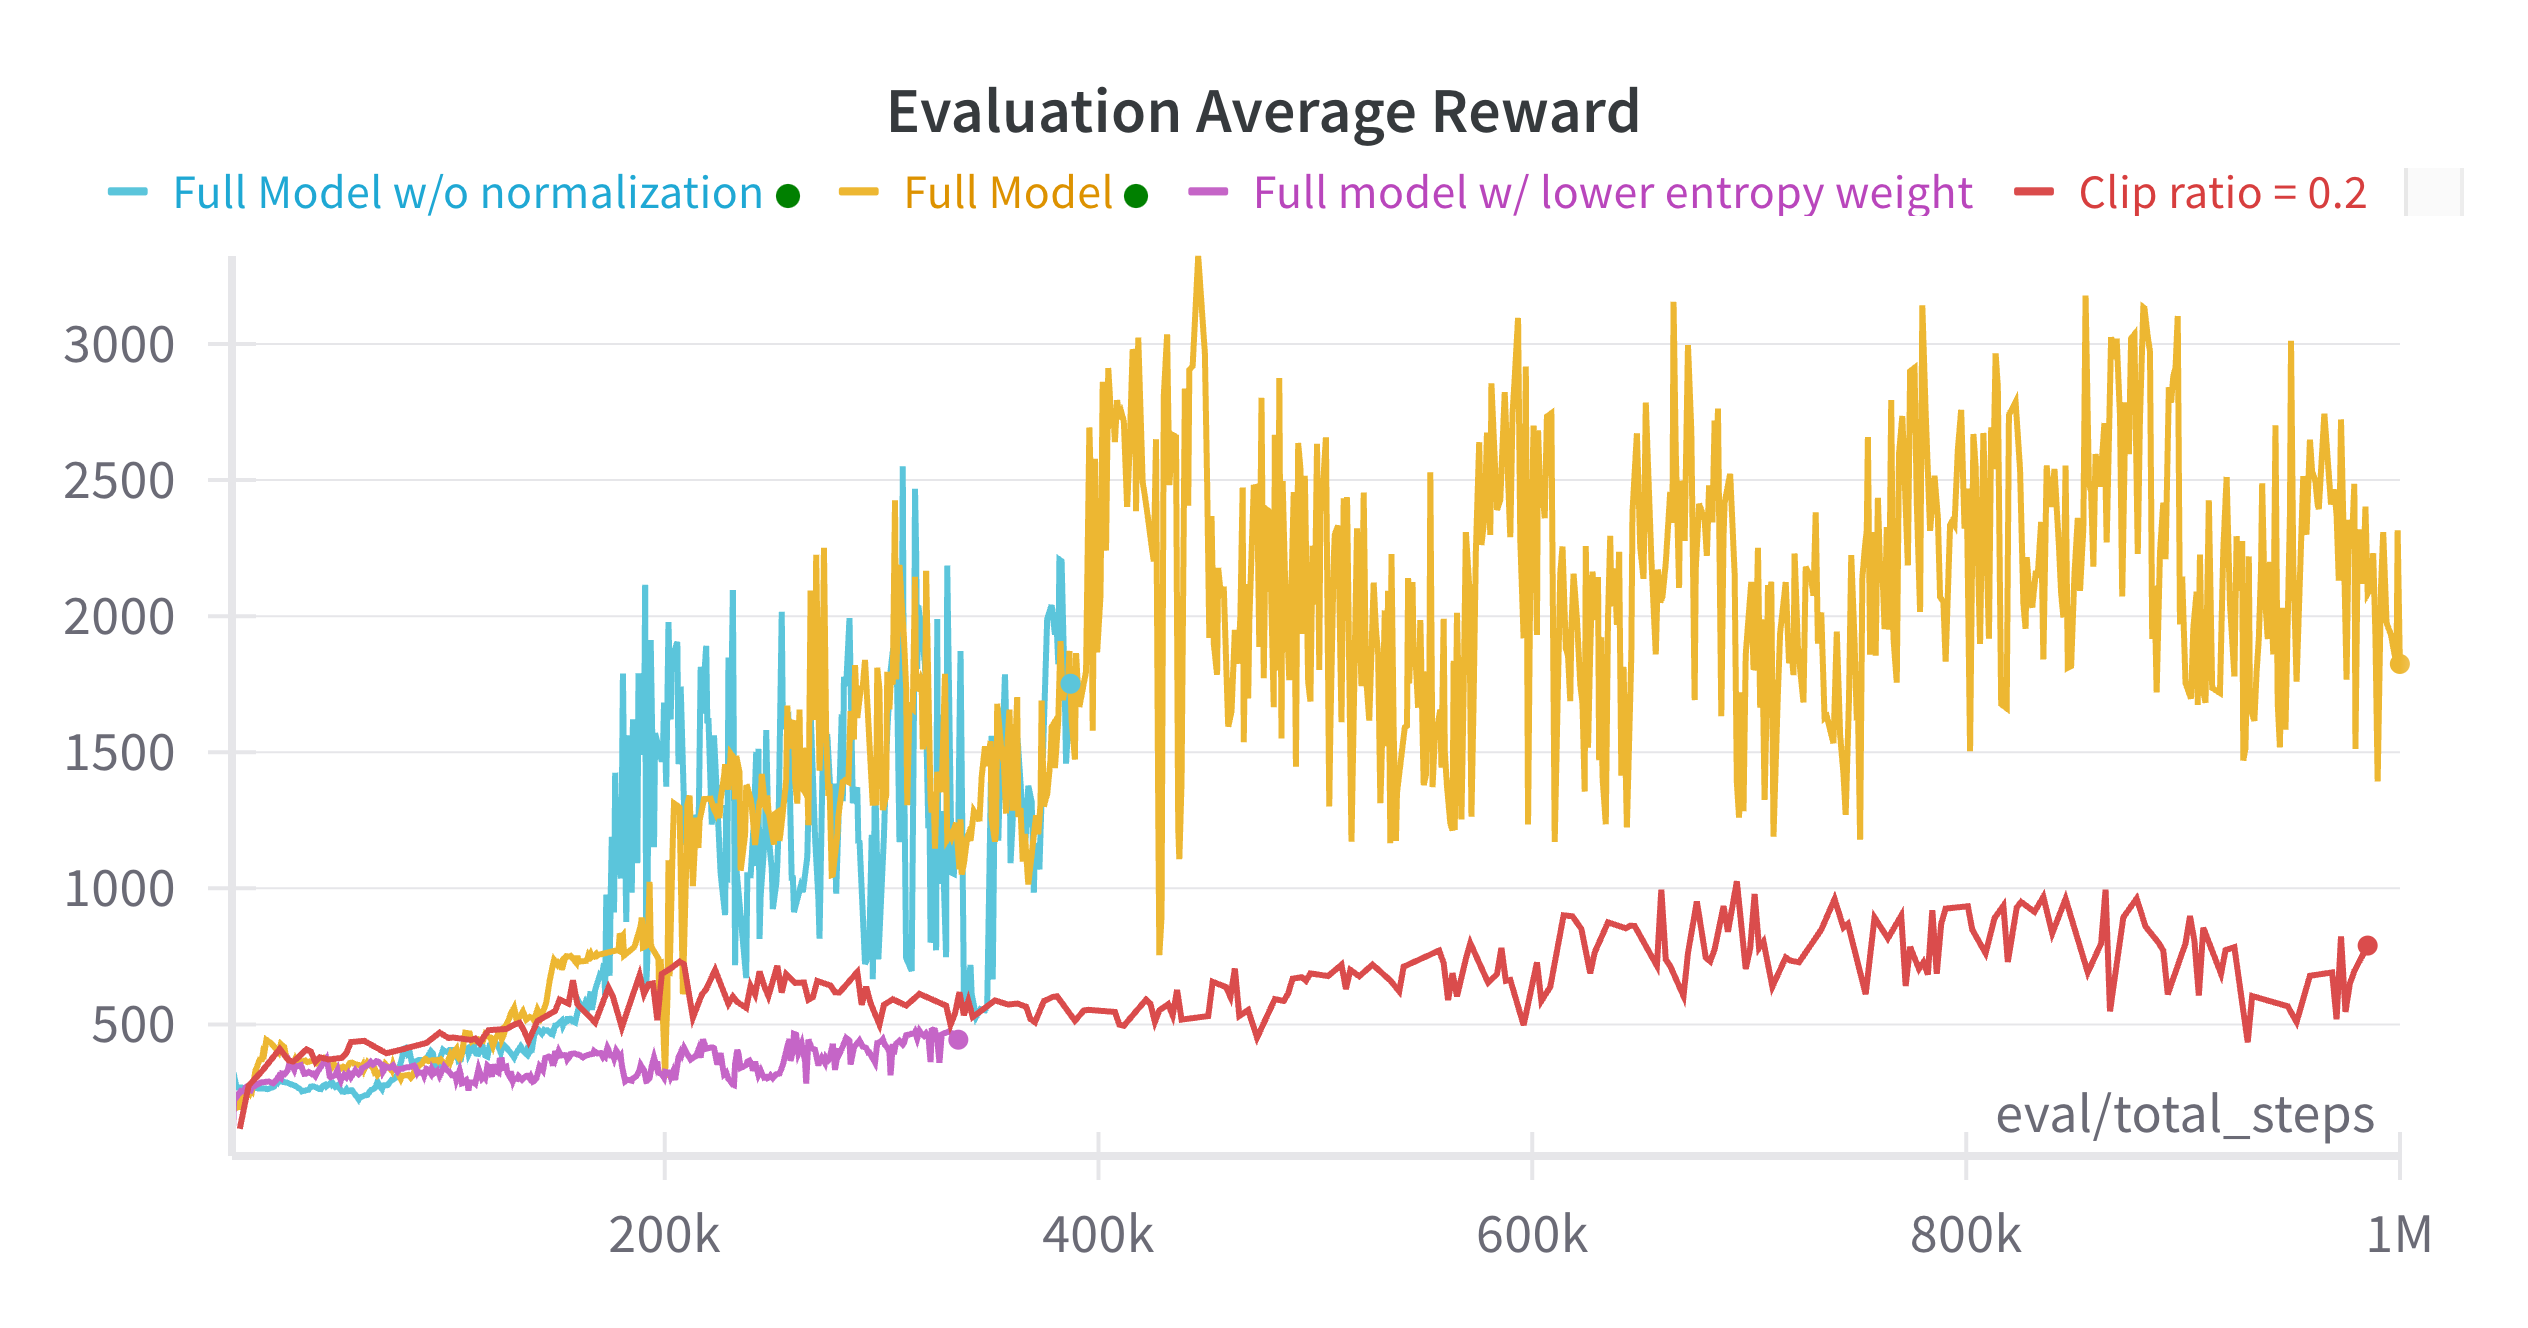
\includegraphics[width=0.95\linewidth]{figures/walker_eval_reward}
\caption{We ablate different parameters, including the clip ratio $\epsilon$ and the entropy weight. We found that only when set the clip ratio to 0.1 and entropy weight to 0.01, the model can get meaningful results. Other two variants fail to achieve higher award, converge at around average episode reward of 400 and 750.}
\label{fig:walkerevalreward}
\end{figure}

\subsubsection{Clipping Parameter}

%\begin{figure}[H]
%\centering
%\includegraphics[width=\linewidth]{clipping_parameter.png}
%\caption{Effect of PPO clipping parameter ($\epsilon$) on training performance in the Pendulum-v1 environment.}
%\label{fig:clipping_parameter}
%\end{figure}

Figure \ref{fig:walkerevalreward} illustrates the impact of different clipping parameter values on PPO's performance in the Walker2d-v4. The clipping parameter ($\epsilon$) controls how much the policy can change in a single update, with larger values allowing for more significant policy shifts.

I experimented with $\epsilon$ values of 0.1 and 0.2 (the default). The results show that:

\begin{itemize}
    \item With $\epsilon = 0.1$ (conservative), learning progresses steadily but somewhat slowly, as the tight constraint on policy updates limits how quickly the policy can improve. However, this setting provides the most stable learning curve with minimal variance.
    
    \item With $\epsilon = 0.2$ (default), the algorithm achieves a good balance between learning speed and stability, converging efficiently to a high-performing policy. This setting reached the target performance at around 150,000 environment steps.
    
\end{itemize}

We find that setting $\epsilon$ to a smaller number leads to a more stable training process. Furthermore, because Walker2d-v4 is a sophiscated locomotion task, I think smaller $\epsilon$ would benifit the training proess, avoiding model collapsing. This is coincided with the experiements results, where smaller $\epsilon$ indeed make the model able to converge to a high score.

\subsubsection{Entropy Coefficient}

Figure \ref{fig:walkerevalreward} shows how different entropy coefficient values affect PPO's performance on the Walker2d-v4 task. The entropy coefficient controls the strength of the entropy bonus, which encourages exploration by rewarding policies with higher entropy (more stochasticity).

I tested entropy coefficients of 0.01 (the value used in my implementation) and 0.005, with the following observations:
\begin{itemize}
	\item With a lower coefficient (0.005), the model fails to achieve meaningful score. I think this mainly due to the lack of exploration in the early phase of training, making the model unable to find the optimal policy and converge around reward of 400.
	\item With a higher coefficient (0.01), our model maintains sufficient exploration throughout the training process, enabling it to discover more effective walking strategies. This increased stochasticity helps the agent escape local optima that might otherwise trap the policy in suboptimal behaviors. The result is significantly better performance, allowing the agent to reach the target reward threshold of approximately 2500. This demonstrates that for complex locomotion tasks like Walker2d-v4, maintaining adequate exploration via higher entropy regularization is crucial for discovering the coordination patterns necessary for stable, efficient walking gaits.
\end{itemize}

These experiments highlight the importance of proper entropy regularization in complex environments like Walker2d-v4. Too little exploration leads to premature convergence to suboptimal behaviors. The value of 0.01 provided the best balance for this specific environment.

It's worth noting that the optimal entropy coefficient differs between environments. For the simpler Pendulum-v1 task, a higher entropy coefficient (0.01-0.05) worked well initially to encourage exploration of the state space, but for Walker2d-v4, a more moderate value (0.005) was more appropriate to balance exploration with the need to refine effective walking behaviors.

\subsection{Additional Analysis: State and Reward Normalization}

%\begin{figure}[H]
%\centering
%\includegraphics[width=\linewidth]{normalization_effect.png}
%\caption{Impact of state and reward normalization on PPO training in the Walker2d-v4 environment.}
%\label{fig:normalization_effect}
%\end{figure}

As an additional analysis, I investigated the effect of state and reward normalization on PPO's performance in the Walker2d-v4 environment. \autoref{fig:walkerevalreward} compares three approaches:

\begin{itemize}
    \item \textbf{No Normalization}: Training without any normalization of states or rewards.    
    \item \textbf{State and Reward Normalization}: Normalizing both observations and rewards.
\end{itemize}

The results demonstrate that:

\begin{enumerate}
    \item Without normalization, training is highly unstable, with large fluctuations in performance. This is due to the widely varying scales of different state dimensions and the sporadic nature of rewards in the Walker environment.
    
    \item Combined state and reward normalization yields the best performance, with the fastest learning and highest final performance. Normalizing rewards helps address the credit assignment problem by creating a more consistent learning signal.
\end{enumerate}

This analysis highlights the importance of proper input normalization for complex control tasks. The Walker2d-v4 environment contains state dimensions that vary significantly in scale (e.g., joint angles vs. velocities) and produces rewards with inconsistent magnitudes. Normalization addresses these issues by ensuring all inputs and learning signals have reasonable and consistent scales.

The improvement from normalization was most noticeable in the early stages of training, where it helped establish stable walking behaviors more quickly. Without normalization, the model often struggled to find initial effective policies, frequently collapsing into local optima where the agent would fall immediately or adopt ineffective movement patterns.

Given these results, I chose to implement both state and reward normalization in my final Walker2d-v4 implementation, which contributed significantly to reaching the target performance of 2,500 reward within the 400K steps.

\section{Conclusion}

In this lab, I implemented and evaluated two policy-based reinforcement learning algorithms, Advantage Actor-Critic (A2C) and Proximal Policy Optimization (PPO) with Generalized Advantage Estimation (GAE), on both the Pendulum-v1 and Walker2d-v4 environments. The experiments yielded several significant findings that demonstrate the advantages of modern policy optimization techniques in continuous control tasks.

The empirical results clearly show that PPO substantially outperforms A2C in terms of sample efficiency and training stability. For the Pendulum-v1 task, PPO required approximately 87\% fewer episodes to reach the threshold reward of -150 compared to A2C, while also achieving a higher final performance. This efficiency gain can be attributed to PPO's ability to perform multiple optimization passes on the same batch of data and its trust region constraint that prevents destructive policy updates.

The ablation studies on key hyperparameters revealed their critical impact on performance. The clipping parameter ($\epsilon$) in PPO provides an essential balance between learning speed and stability, with the value of 0.1 yielding the most robust results for the Walker2d-v4 environment. Similarly, the entropy coefficient proved crucial for maintaining adequate exploration, particularly in complex environments where premature convergence to suboptimal behaviors is a significant risk.

For the challenging Walker2d-v4 environment, normalization techniques played a vital role in achieving high performance. The combination of state and reward normalization significantly enhanced learning stability by addressing the varying scales of state dimensions and creating more consistent learning signals, ultimately enabling the agent to reach an average evaluation score of around 2500 within 400K environment steps.

This implementation and analysis demonstrate how modern policy optimization methods like PPO can effectively solve complex locomotion tasks with continuous action spaces. The improved stability mechanisms introduced by PPO—particularly the clipped surrogate objective and generalized advantage estimation, providing practical solutions to the challenges inherent in policy gradient methods. These approaches strike a balance between exploration and exploitation while ensuring controlled policy updates, resulting in more reliable and sample-efficient learning across different control tasks.



\printbibliography
\end{document}